\chapter{減算型表示を用いたプロトタイプの実装}
\label{chapter:implement_dr}
本章では,減算型表示用いて実装したプロトタイプについて述べる.

\section{システムの概要}
  減算型表示を用いたシステムのプロトタイプは,モバイルデバイス上で実行できるようUnity(ver 5.6.0f3)を用いてC\#言語で実装した.
  実環境に近づけるために,RECOH THETA\footnote{\url{https://theta360.com/}(2017/4/27確認)}を用いて新日本新地ビル付近で撮影した昼と夜の全天球画像(図\ref{figure:kitashinchi_day},\ref{figure:kitashinchi_night})を用意し,モバイルデバイスを通して見回せるようにした.全天球画像では看板が鮮明に撮影できないため,看板は別に撮影した画像をオブジェクトとして設置した.

  実験に用いる看板情報は,図\ref{fig:kitashinchi} - (a) に示す大阪府北新地の新日本新地ビルに掲示されている61枚の看板を用いた.店舗の種類は株式会社キックによる北新地総合情報サイト\footnote{\url{http://kgnet.jp/}(2017/4/27確認)}を参考に,「スナック・ラウンジ」,「バー」,「和食」,「居酒屋」,「クラブ」,「寿司」,「中華料理」,「ドレスショップ」の8種類に分類した.サイトに記載がなかった店舗は,「その他」として分類した.データベースはシステムから容易に参照できるようにするために,リレーショナルデータベースであるSQLite\footnote{\url{https://www.sqlite.org/}(2017/4/27確認)}(ver 3.8.10.2)を用いて,画像内の看板の位置,店舗の名前,店舗の種類,看板画像をそれぞれ格納した.

  \begin{figure}[tb]
    \begin{center}
      \begin{tabular}{c}
        \begin{minipage}[t]{.95\hsize}
          \centering
          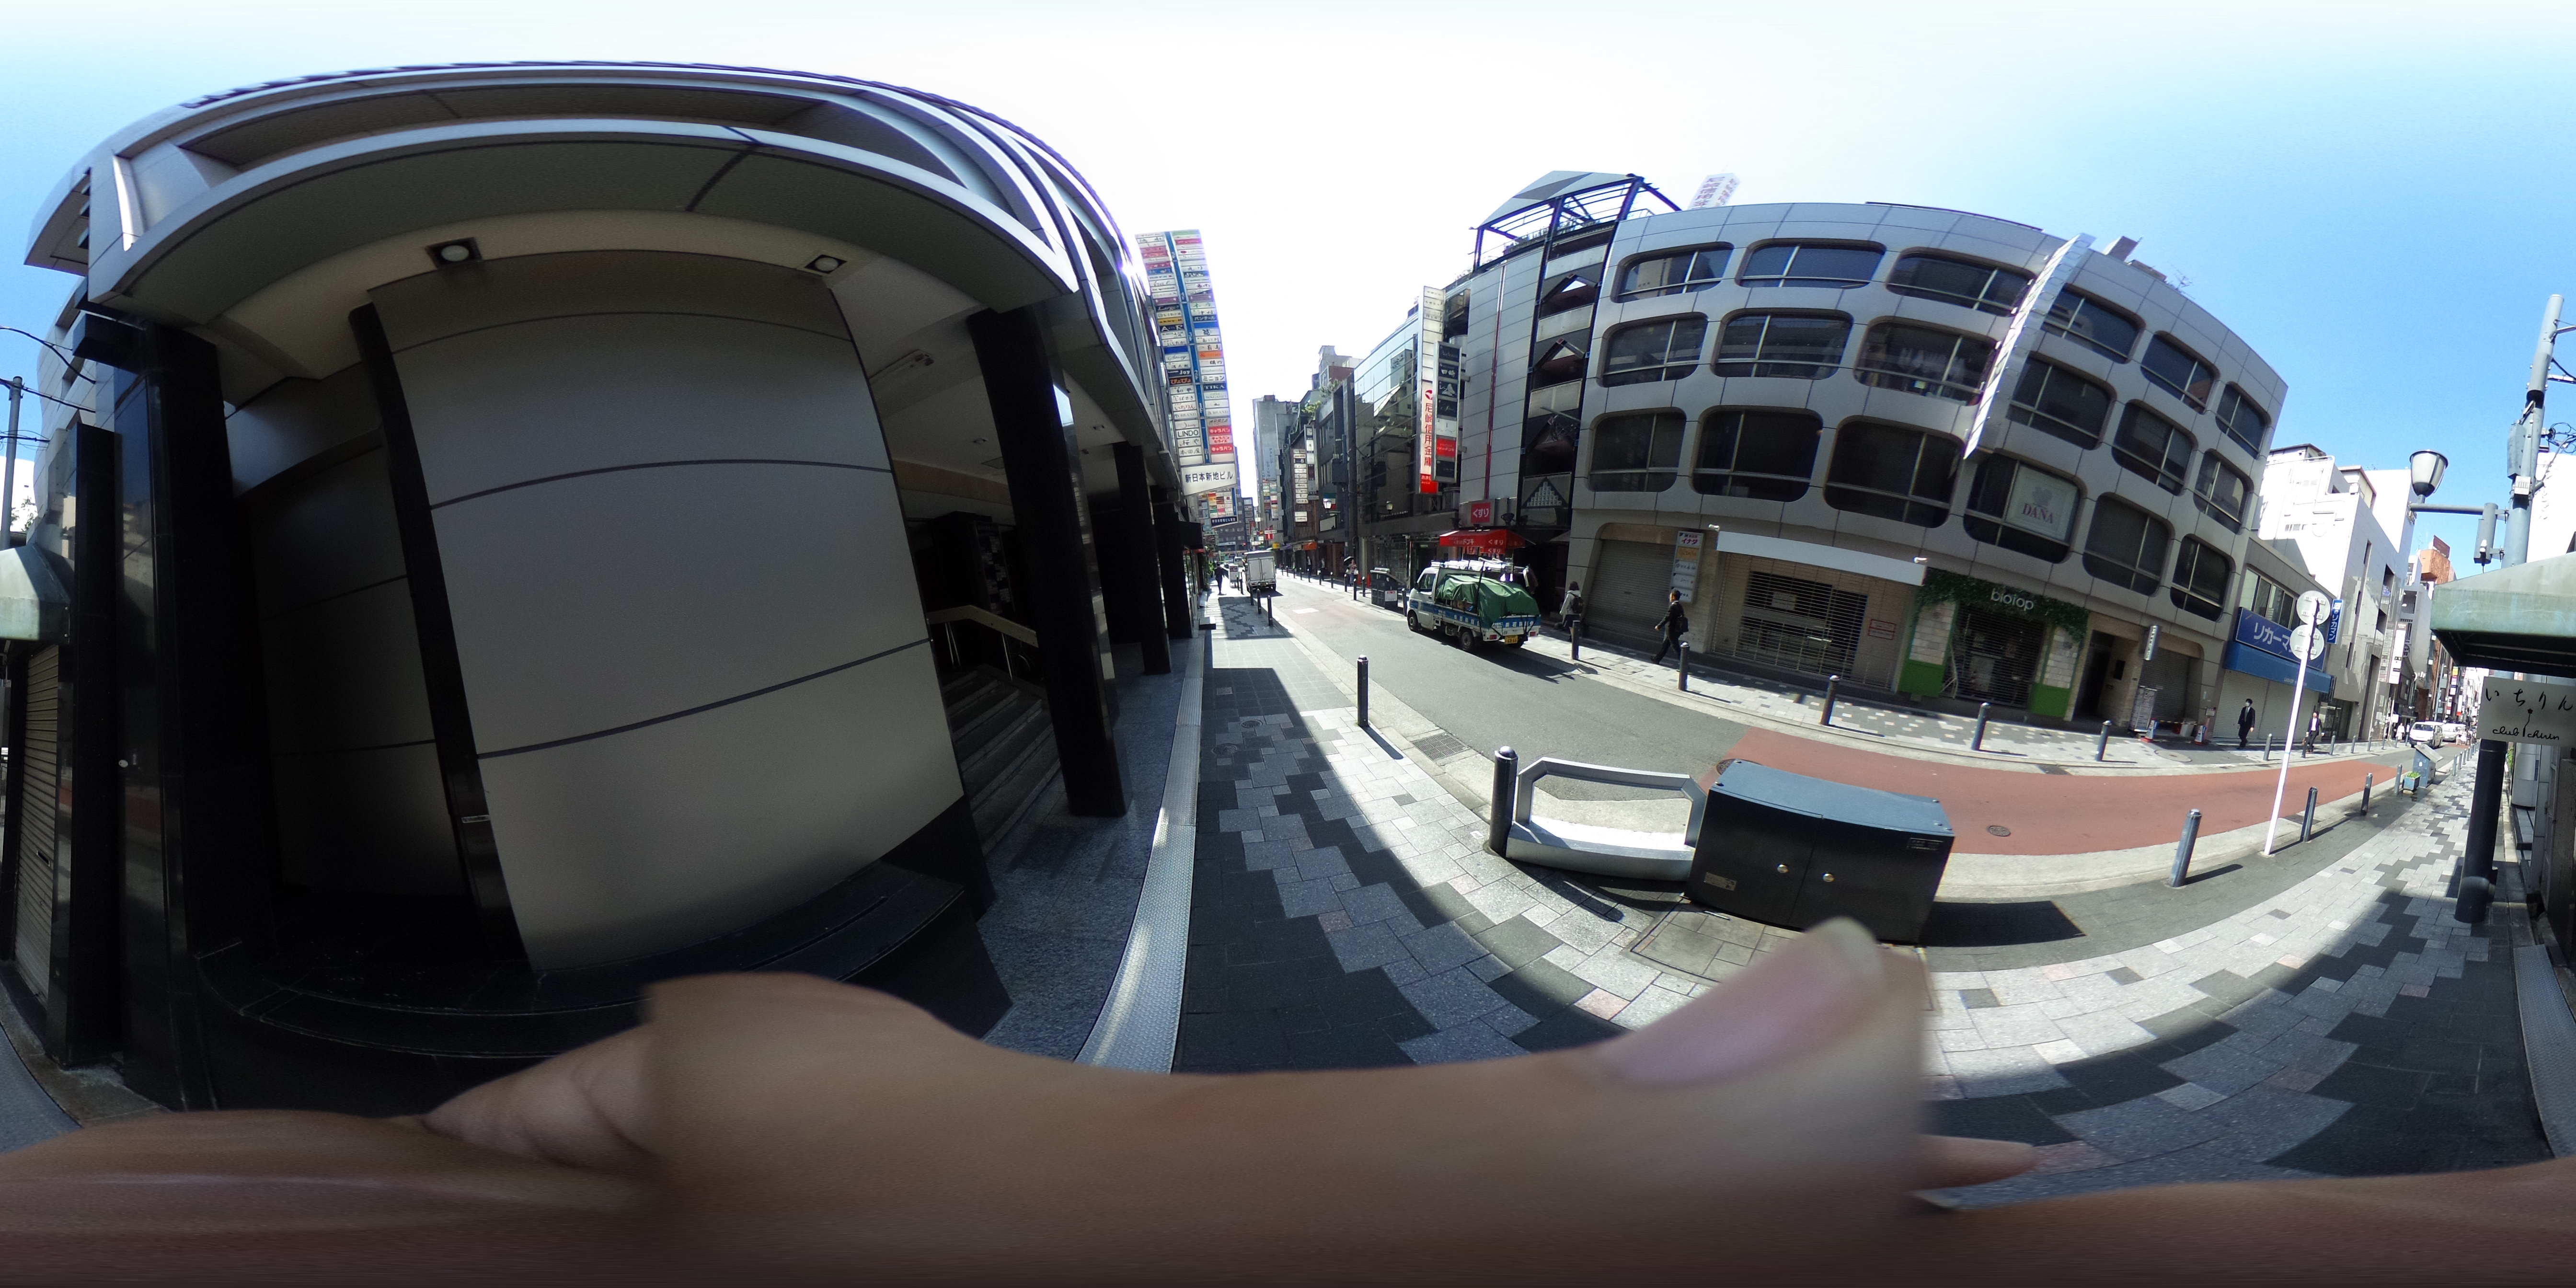
\includegraphics[width=\columnwidth, clip]{kitashinchi_day.jpg}
          \caption{プロトタイプで用いる環境(昼)}
          \label{figure:kitashinchi_day}
        \end{minipage} \\ \\
        \begin{minipage}[t]{.95\hsize}
          \centering
          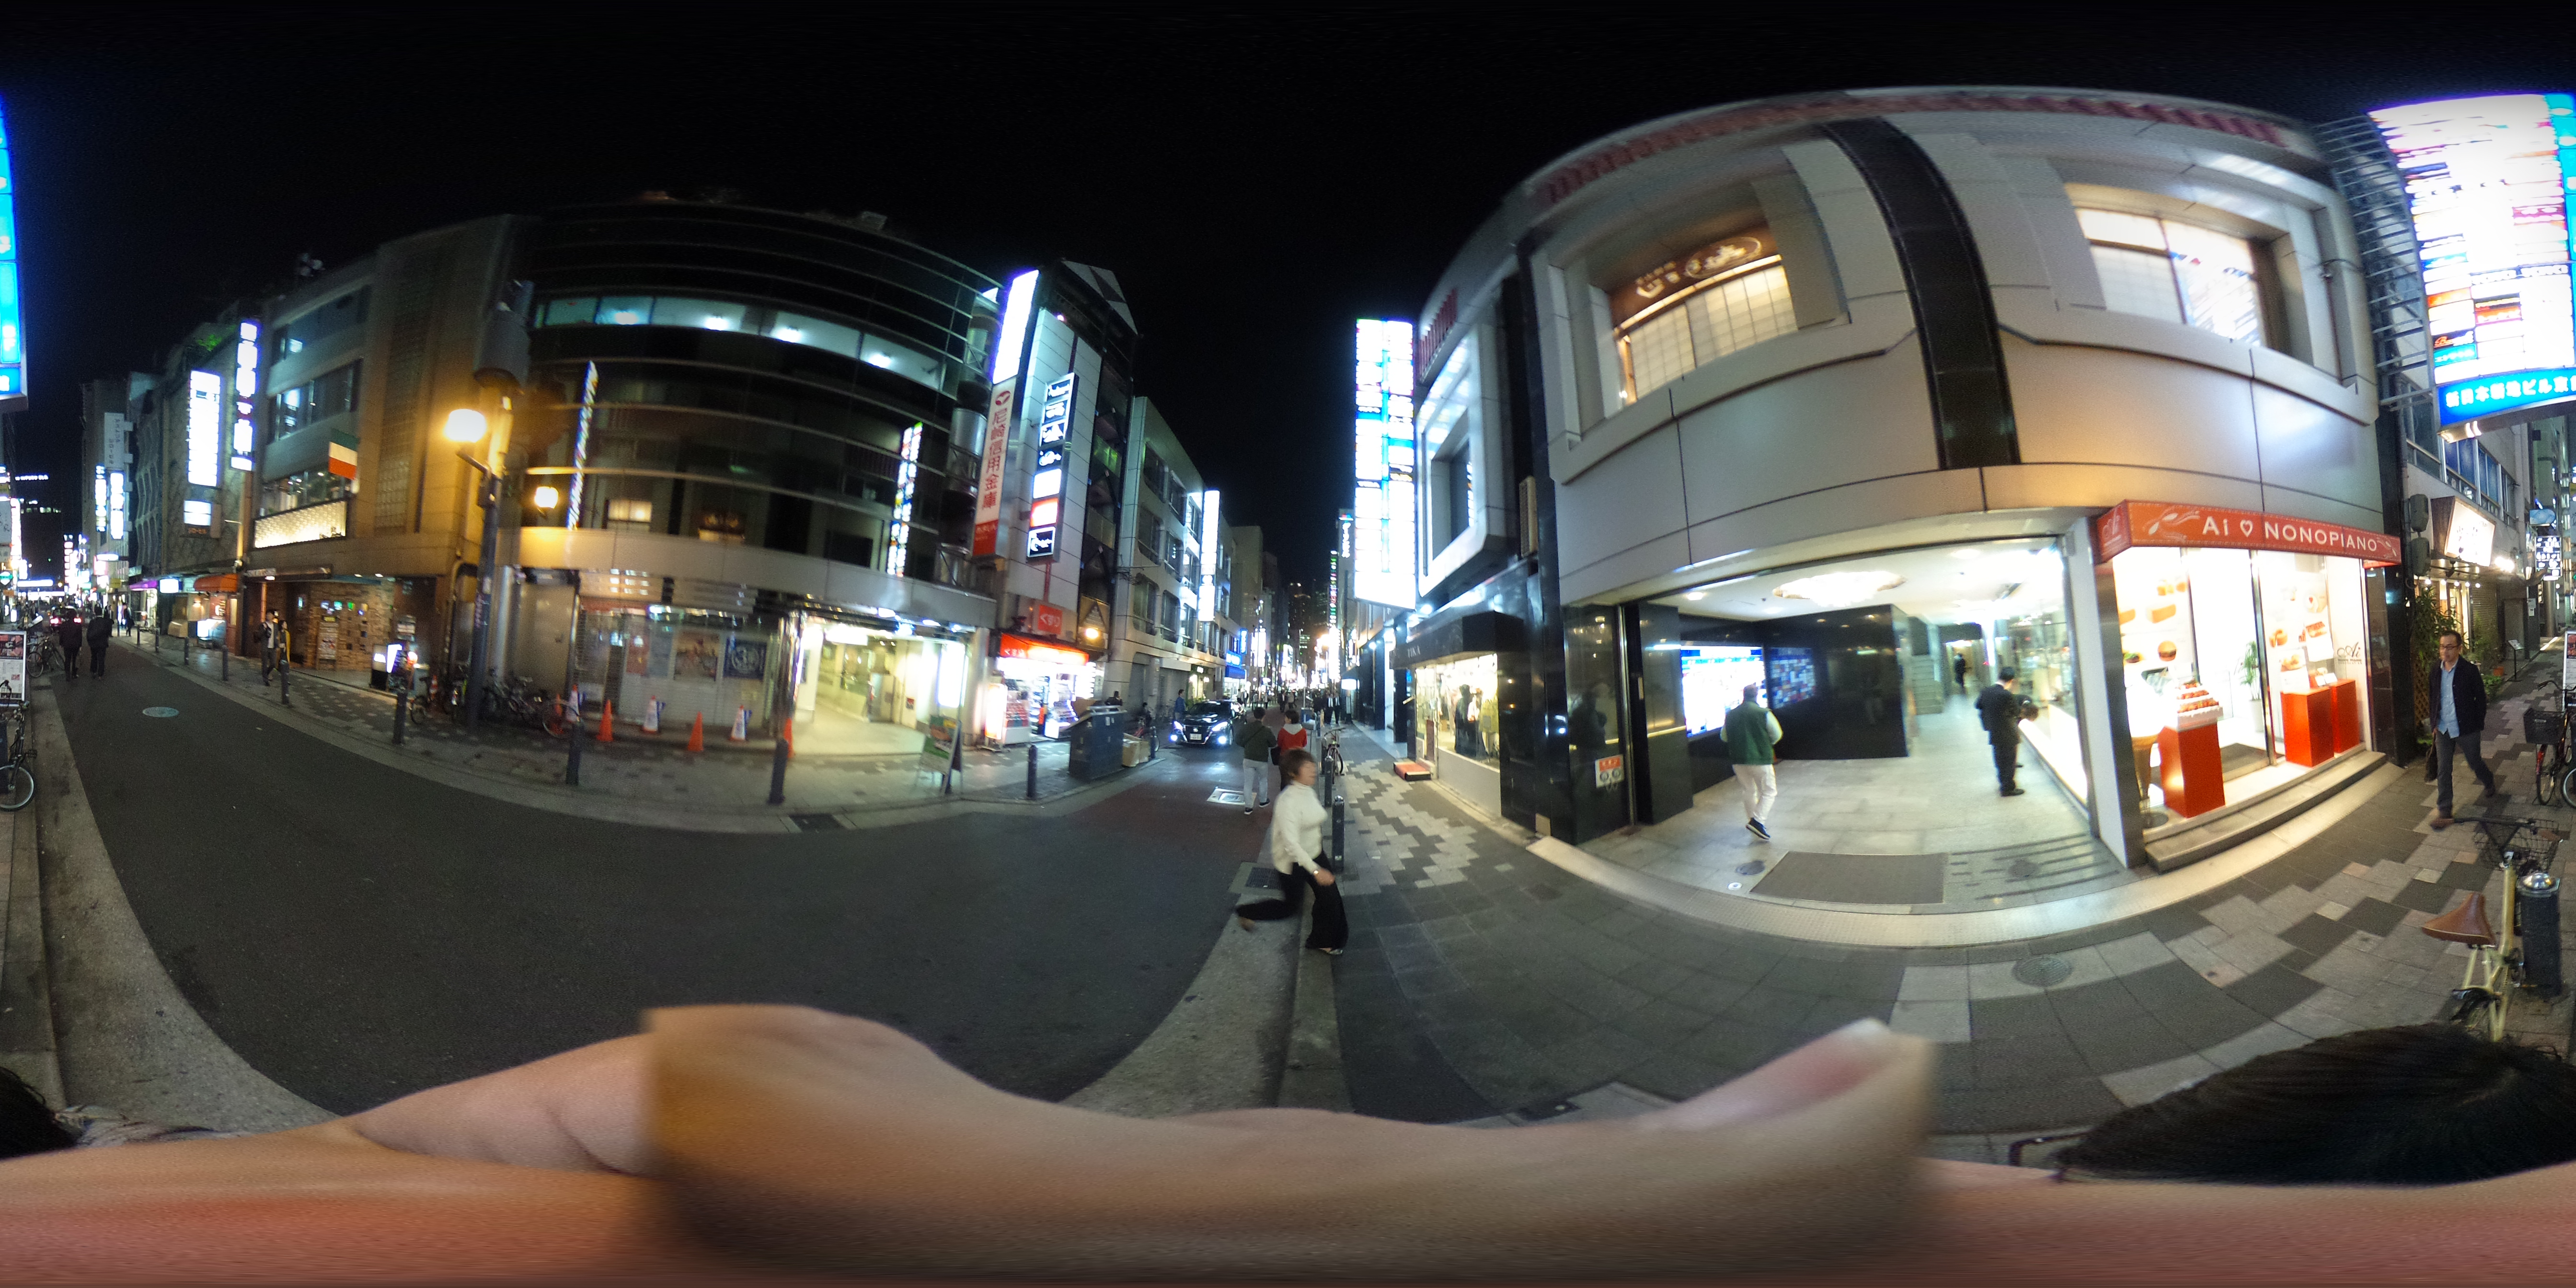
\includegraphics[width=\columnwidth, clip]{kitashinchi_night.jpg}
          \caption{プロトタイプで用いる環境(夜)}
          \label{figure:kitashinchi_night}
        \end{minipage}
      \end{tabular}
    \end{center}
  \end{figure}


\section{システムの動作}
  プロトタイプでは,ユーザはモバイルデバイスを全天球画像内で全方向に向けることができる.システムは画面中央のローカル座標と看板のワールド座標を対応させることにより,画面中央と看板を重ね合わせると特定の看板が選択されたことを認識できる.情報提示手法に関しては,
  \begin{itemize}
    \item 加工なし(以下,通常型と記す)
    \item 看板の横に店舗名を表示(図\ref{fig:prototype} -(a),以下,加算型と記す)
    \item 特定の看板以外の情報をグレースケール化(図\ref{fig:prototype} -(b),以下,減算型と記す)
    \item 特定の看板以外の情報をグレースケール化し,看板の横に店舗名を表示(図\ref{fig:prototype} -(c),以下,ハイブリッド型と記す)
  \end{itemize}
  の4種類を切り替えられるようにし,探索対象の看板は,店舗の種類別に切り替えられるようにした.プロトタイプのインタフェースを図\ref{figure:dr_interface}に示す.また,ユーザがスタートボタンをタップしてから特定の看板を見つけるまでの所要時間を計測できる機能を用意した.ユーザが特定の看板に画面の中央を1秒間合わせると,看板を見つけたと判定するよう実装した.

  \begin{figure}[t]
    \begin{center}
      \begin{tabular}{ccc}
        \begin{minipage}{0.3\hsize}
          \centering
          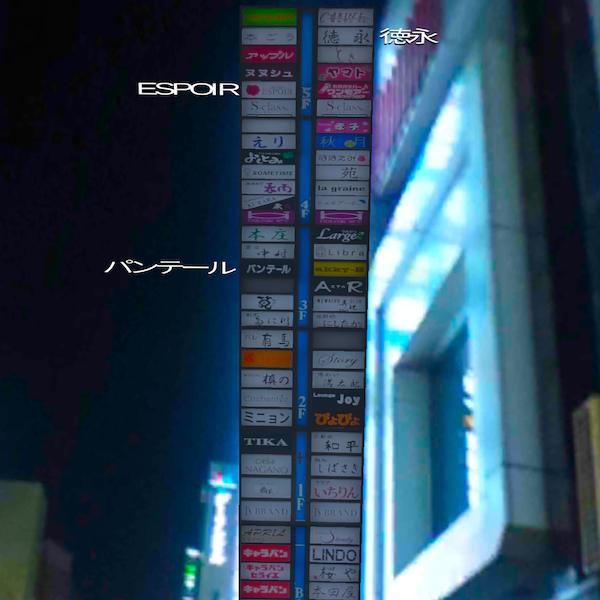
\includegraphics[clip, width=.95\textwidth]{dr_method1.png}\\
          \small{(a)加算型}
        \end{minipage}
        \begin{minipage}{0.3\hsize}
          \centering
          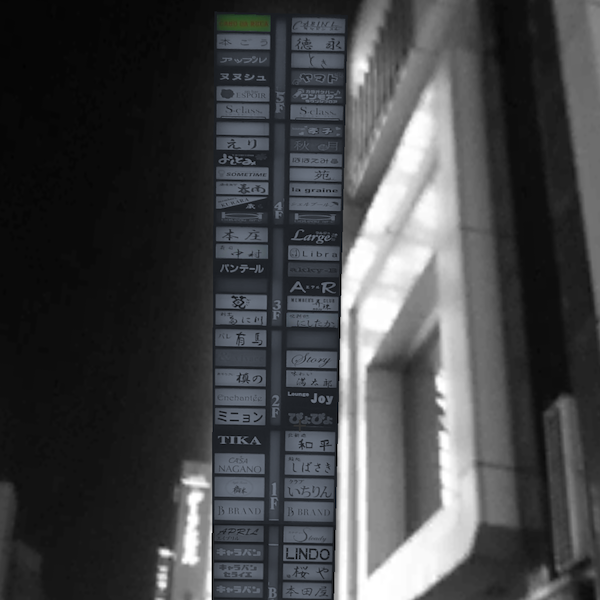
\includegraphics[clip, width=.95\textwidth]{dr_method2.png}\\
          \small{(b)減算型}
        \end{minipage}
        \begin{minipage}{0.3\hsize}
          \centering
          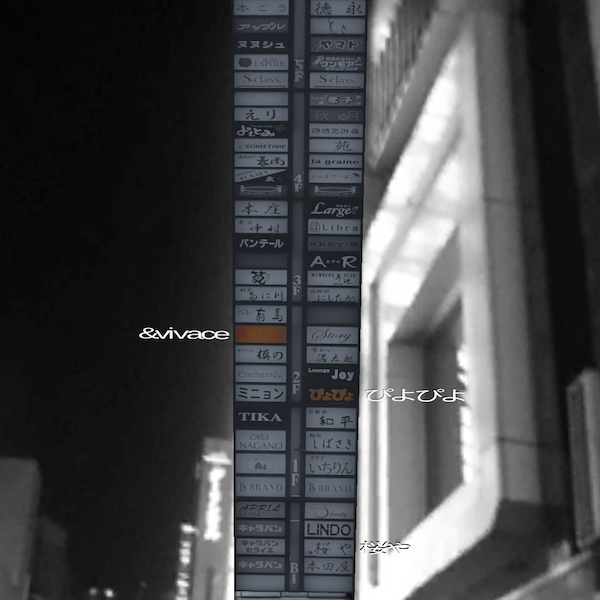
\includegraphics[clip, width=.95\textwidth]{dr_method3.png}\\
          \small{(c)ハイブリッド型}
        \end{minipage}
      \end{tabular}
      \caption{プロトタイプの出力画面}
      \label{fig:prototype}
    \end{center}
  \end{figure}
  \begin{figure}[tb]
    \centerline{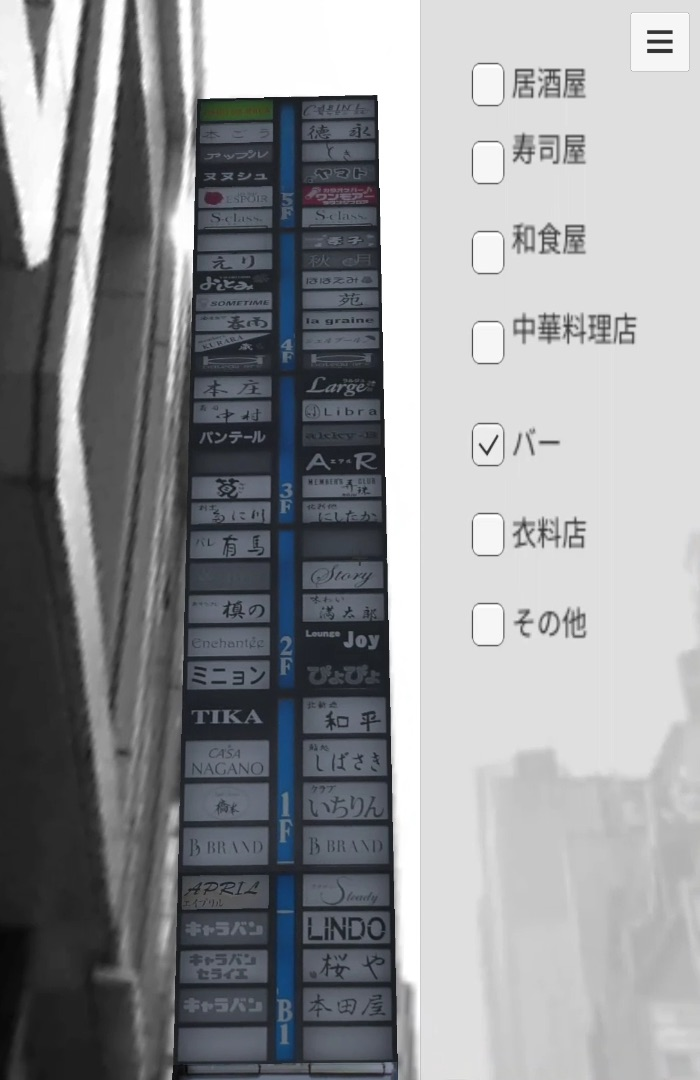
\includegraphics[width=.65\columnwidth, clip]{dr_interface.jpg}}
    \caption{プロトタイプのインタフェース}
    \label{figure:dr_interface}
  \end{figure}
